%% ****** Start of file aiptemplate.tex ****** %
%%
%%   This file is part of the files in the distribution of AIP substyles for REVTeX4.
%%   Version 4.2 of December 2014.
%%
%
% This is a template for producing documents for use with 
% the REVTEX 4.2 document class and the AIP substyles.
% 
% Copy this file to another name and then work on that file.
% That way, you always have this original template file to use.

\documentclass{article}
%\documentclass[aip,reprint]{revtex4-2}

\usepackage{graphicx}% Include figure files
\usepackage{dcolumn}% Align table columns on decimal point
\usepackage{bm}% bold math
\usepackage{amsmath}
\usepackage{amssymb}{}
\usepackage{caption, subcaption}
\usepackage{usual}
\usepackage{array}

\renewcommand{\Re}{\mathrm{Re}}
\renewcommand{\Im}{\mathrm{Im}}
\newcommand{\Th}{\mathrm{Th}}

\begin{document}

% Use the \preprint command to place your local institutional report number 
% on the title page in preprint mode.
% Multiple \preprint commands are allowed.
%\preprint{}
%

% repeat the \author .. \affiliation  etc. as needed
% \email, \thanks, \homepage, \altaffiliation all apply to the current author.
% Explanatory text should go in the []'s, 
% actual e-mail address or url should go in the {}'s for \email and \homepage.
% Please use the appropriate macro for the type of information

% \affiliation command applies to all authors since the last \affiliation command. 
% The \affiliation command should follow the other information.


% Collaboration name, if desired (requires use of superscriptaddress option in \documentclass). 
% \noaffiliation is required (may also be used with the \author command).
%\collaboration{}
%\noaffiliation

% \date{\today}



\section{General picture}

In amplifier terminology, $\alpha$ refers to a dimensionless 'intra-cavity light strength', which can be understood as a semiclassical treatment of of bosonic annihilation operator $a$. i.e. $|\alpha|^2$ stands for 'intra-cavity photon number'. 

A problem is that the term 'intra-cavity' is actually ill defined. We kind of understand the interior of a 3D cavity, or a Fabry-Perot like structure (e.g. TL with capacitors on both sides). While generally speaking, a mode doesn't have to be confined in particular spatial region with clear geometric boundaries. A \emph{mode} stands for the eigenvalue (frequency) and eigenvector (field distribution function) for Maxwell Eqs with certain boundary condition, which I interprete as the 'undriven' EM field allowed in the system. Strictly speaking, the term 'intra-cavity' refers to photon occupation of the EM field structure corresponding to a particular mode, which has no physical meaning at off-resonance (non-eigenvalue) frequencies. 

Instead of photon number existing within certain spatial region, a better quantity we can always count on is photon flux (photon number per unit time) that flows through a certain cross section. The photon scattering picture stands for light at whatever frequency. All we need to do then is to determine a particular cross section in evaluating photon flux and be consistant with the choice. 

In our superconducting circuit system, Josephson elements, which provides nonlinearity for the system, are of key importance. While Josephson relation has an easy expression in terms of electric current and superconducting phase, describing a Josephson junction in photon scattering language is much less familiar to us (at least to me). 

Therefore, in the following I'm going to simply describe the whole system in electrical language instead of microwave photon scattering language. 

Josephson relation links current $I(t)$ to the superconducting phase $\varphi(t) = \Phi(t)/\phi_0$ across a JJ. Put it more general to other Josephson elements such as a SNAIL, which can always be expressed in a nonlinear potential such as: 

\begin{equation}
U =E_j \( c_0 + \frac{c_2}{2!} \tilde{\varphi}^2 + \frac{c_3}{3!} \tilde{\varphi}^3 + \frac{c_4}{4!} \tilde{\varphi}^4 + \cdots\)
\end{equation}
and therefore a current-flux relation: 
\begin{equation}
I = \frac{E_j}{\phi_0} \( c_2\tilde{\varphi} +  \frac{c_3}{2} \tilde{\varphi}^2  + \frac{c_4}{6} \tilde{\varphi}^3 + \cdots \)
\end{equation}

The size of Josephson elements in a circuit are usually much smaller compared to microwave wavelength, allowing us to treat them as lumped elements (except for the case of Josephson transmission-line). For simplicity, let's assume there's only one Josephson element in the circuit and it's a dipole-like element (two terminals). The EM environment seen by the Josephson element will include the linear response of the circuit excluding the JJ, all the loadings, and all possible external drives. According to Thevenin theorem, such a linear one-port (two terminals) network can always be represented by an equivalent impedance $Z^{\Th}[\omega]$ and an equivalent voltage source $V^{\Th}(t)$ in series. 

\begin{figure}[htb]
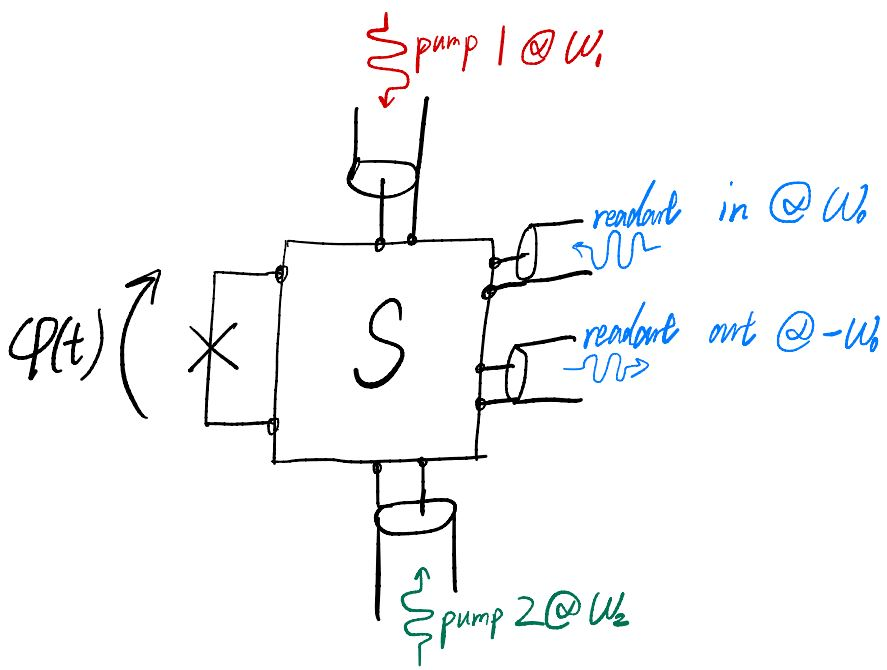
\includegraphics[width=10cm]{figures/general_picture.jpg}
\caption{JJ and several input/output channels (ports)}
\end{figure}

In the cases of interest, our external drives always consist of discrete frequency harmonic components, say $\omega_s$, $\omega_i$, $\omega_p$ etc. So linear response theory (applied on the Thevenin circuit) guarantees that $V^{\Th}(t)$ also have only these harmonic components. i.e.

\begin{equation*}\label{eq:VTh}
V^{\Th}(t) = \Re \( V^{\Th}_{\omega_s} \exp{j\omega_s t} + V^{\Th}_{\omega_p} \exp{j\omega_p t} + V^{\Th}_{\omega_i} \exp{j\omega_i t} \)
\end{equation*}
where we have used the phasor representation. And similarly we can write the resulting current as: 

\begin{equation*}
\begin{aligned}
	I(t) &= \Re \( I_{\omega_s} \exp{j\omega_s t} + I_{\omega_p} \exp{j\omega_p t} + I^*_{\omega_i} \exp{-j\omega_i t} \) \\
	&= \frac{1}{2} \( I_{\omega_s} \exp{j\omega_s t} + I_{\omega_p} \exp{j\omega_p t} + I^*_{\omega_i} \exp{-j\omega_i t} + I^*_{\omega_s} \exp{-j\omega_s t} + I^*_{\omega_p} \exp{-j\omega_p t} + I_{\omega_i} \exp{j\omega_i t}
	 \)
\end{aligned}
\end{equation*}

As mentioned before, another dynamical variable we want to look at is phase across the Josephson element: 
\begin{equation*}
\begin{aligned}
	\tilde{\varphi}(t) &= \Re \( \varphi_{\omega_s} \exp{j\omega_s t} + \varphi_{\omega_p} \exp{j\omega_p t} + \varphi^*_{\omega_i} \exp{-j\omega_i t} \) \\
	&= \frac{1}{2} \( \varphi_{\omega_s} \exp{j\omega_s t} + \varphi_{\omega_p} \exp{j\omega_p t} + \varphi^*_{\omega_i} \exp{-j\omega_i t} + 
	\varphi^*_{\omega_s} \exp{-j\omega_s t} + \varphi^*_{\omega_p} \exp{-j\omega_p t} + \varphi_{\omega_i} \exp{j\omega_i t}
	 \)
\end{aligned}
\end{equation*}

Or equivalently, voltage drop on the Josephson element, whose harmonic components are simply: 
\begin{equation*}
V_\omega = j \omega \phi_0 \varphi_\omega
\end{equation*}

\begin{figure}[htb]
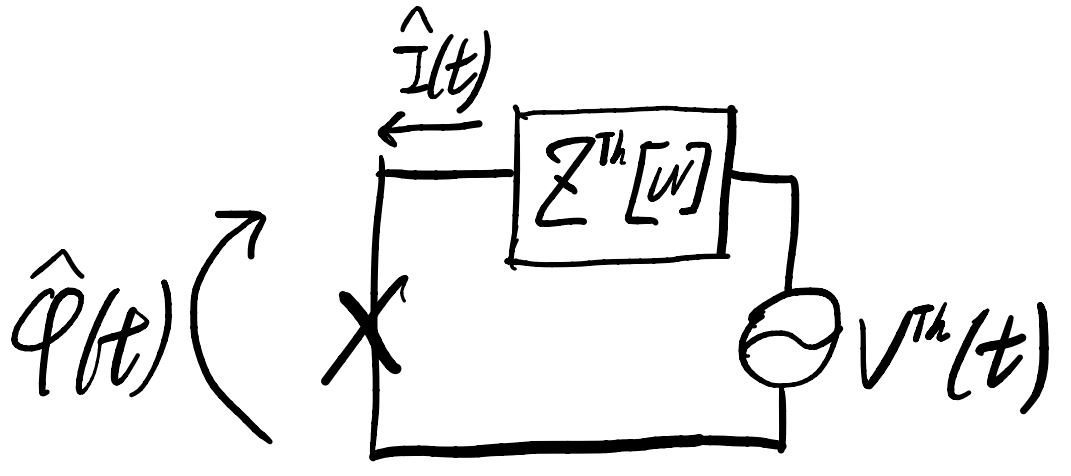
\includegraphics[width=7cm]{figures/Thevenin.jpg}
\caption{Thevenin equivalent circuit for the environment seen by the JJ}\label{fig:Thevenin}
\end{figure}

The whole system will satisfy: 

\begin{equation}
	I_{\omega} Z^\Th[\omega] + V_{\omega} = V^\Th_\omega 
\end{equation}

The only tricky part is that the Josephson response between $I_{\omega}$ and $V_{\omega}$ is nonlinear. For example, considering the $c_3$ term in SNAIL potential, different harmonic components are linked by: 
\begin{equation}
	I_{\omega_s} = \frac{E_j}{\phi_0} \(c_2 \varphi_{\omega_s} + \frac{c_3}{2} \varphi_{\omega_p} \varphi^*_{\omega_i}\) 
\end{equation}


($\omega_p = \omega_s + \omega_i$ in typical amplifier terminology)



A general treatment is to put the above equations at all relavent harmonic components together, and solve them all self-consistently. This method is called 'harmonic balance' calculation. 


However, in some easy but common cases, we can assume one or several of the harmonic components to be 'stiff', i.e. a drive being strong enough that the responding strength at that frequency is almost indepent of the other harmonic components. Strictly speaking $\varphi_{\omega_p}, \varphi_{\omega_s}, \varphi_{\omega_i}$ values are linked to each other in the nonlinear dynamicalnamics, but the fluctuation in $\varphi_{\omega_p}$ is much less than its steady value induced by the external pump, we say the pump is stiff and simply take $\varphi_{\omega_p}$ as fixed (corresponding to pump strength).

In this case, we can evaluate the steady linear response $\varphi_{\omega_p}$ independent of what happens at $\omega_s$ and $\omega_i$. Then, using this $\varphi_{\omega_p}$ as a parameter, we joyfully realize that the Josephson response at the other frequencies can also be linearized. This trick was introduced as 'pumpistor model'. 

E.g. we can write
\begin{equation}
\begin{aligned}
Y_J[\omega_s] &= \frac{I_{\omega_s}}{V_{\omega_s}}\\
&= \frac{1}{j\omega_s L_J} + \frac{\frac{c_3 \varphi_{\omega_p}}{2c_2} }{j\omega_s L_J}\frac{ \varphi^*_{\omega_i}}{\varphi_{\omega_s}}
\end{aligned}
\end{equation}
($L_J = \frac{\phi^2_0}{E_j c_2}$ is the total Josephson inductance) 

Combined with similar relation at $-\omega_i$, we arrive at: 
\begin{equation}
\(
\begin{matrix}
I_{\omega_s}\\
I^*_{\omega_i}
\end{matrix}
\)
= 
\frac{1}{j L_J}
\(
\begin{matrix}
\frac{1}{\omega_s} & \frac{\epsilon}{-\omega_i}\\
\frac{\epsilon^*}{\omega_s} & \frac{1}{-\omega_i}
\end{matrix}
\)
\(
\begin{matrix}
V_{\omega_s}\\
V^*_{\omega_i}
\end{matrix}
\)
\end{equation}
where we named $\epsilon = \frac{c_3\varphi_{\omega_p}}{2c_2}$

This is the linearized response of a 3-wave-mixing Josephson element under stiff pump. 

We might also want to include 4th order nonlinearity, i.e. Kerr effect due to $\varphi_{\omega_p}$ (while unfortunately, in pumpistor model we can not include Kerr effect due to $\varphi_{\omega_s}$ itself in the dynamics at $\omega_s$).

And strictly speaking, we should always include all 'relavent' frequency components linked by the stiff $\varphi_{\omega_p}$. E.g. the frequency $\omega_h = \omega_s + \omega_p$ enters the nonlinear dynamics for $\omega_s$ in lowest order, so it should be included, even if we're not driving nor measuring at that frequency. 

What we get is: 
\begin{equation}
	I_{\omega_s} = I_c \(c_2 \varphi_{\omega_s} + \frac{c_3}{2} \( \varphi_{\omega_p} \varphi^*_{\omega_i} + \varphi^*_{\omega_p} \varphi_{\omega_h}\) + \frac{c_4}{4} |\varphi_{\omega_p}|^2 \varphi_{\omega_s}\) 
\end{equation}

And resulting linearized response: 

\begin{equation}
\(
\begin{matrix}
I_{\omega_s}\\
I^*_{\omega_i}\\
I_{\omega_h}
\end{matrix}
\)
= 
\frac{1}{j L_J}
\(
\begin{matrix}
\frac{1 + \delta}{\omega_s} & \frac{-\epsilon}{\omega_i} & \frac{\epsilon^*}{\omega_h}\\
\frac{-\epsilon^*}{\omega_s} & \frac{1 + \delta}{\omega_i} & 0 \\
\frac{\epsilon}{\omega_s} & 0 & \frac{1 + \delta}{\omega_h}
\end{matrix}
\)
\(
\begin{matrix}
V_{\omega_s}\\
V^*_{\omega_i}\\
V_{\omega_h}
\end{matrix}
\)
\end{equation}
which we should put together with: 
\begin{equation*}
\begin{aligned}
	I_{\omega_s} Z^\Th[\omega_s] + V_{\omega_s} &= V^\Th_{\omega_s} \\
	I^*_{\omega_i} Z^\Th[-\omega_i] + V^*_{\omega_i} &= V^{\Th^*}_{\omega_i}  \\
	I_{\omega_h} Z^\Th[\omega_h] + V_{\omega_h} &= 0
\end{aligned}
\end{equation*}
and solve self-consistently (now as a linear system, this calculation is much easier than harmonic balance and we can expect some closed form expressions for the results). 


\begin{itemize}
	\item Engineering efficient pump coupling is equivalent to engineering a linear network in figure 1 that enables sufficient $\varphi_{\omega_p}$ with less input power from the physical port. 

This converts to two questions for the Thevenin circuit: 

1. What properties do we want of $Z^\Th[\omega]$? 

2. How do the pumps from physical ports go into $V^\Th$? 

(My work on PPFSPA was trying to answer these questions for a specific application, i.e. a JPA with two external ports. )

\item Engineering the gain profile of an amplifier. Amplifers should have $|S_{11}[\omega]| > 1$ satisfied for a decent range of $\omega$. Usual resonance-based parametric amplifiers typically shows a Lorentzian lineshape gain profile versus frequency, and have a gain-bandwidth tradeoff. While this can be improved by engineering the linear coupling network. 


\item Figure out how noise (unexpected voltage sources at all possible frequencies) affects the SNR we care about. On one hand, we'd like to know the added noise performance for our parametric processes, e.g. guarantee it's quantum limited. On the other hand, we can intentionally make our system more susceptible or less susceptible to certain frequency noise from certain input channels (physical ports). Noise spectrometry, and offer instructions on line attenuation and filering. 

\item A more systematic approach of describing the system is always favored, especially as we have multiple requirements on a single module (?) and as we afford having more complex systems our single module. 

Instead of starting the design from minimal 'atoms', perhaps we'll start with some overall requirements on the system response function, controlability, observability etc. 

Knowing what macroscopic properties we want, how to achieve that with basic circuit building blocks (such as L, C, TL) can become an optimization problem. 

\end{itemize}




\newpage
\section{Evaluate flux induced by the external drive}

Apart from simulation (which is more for analyzing than synthesizing), I found a method called the 'signal flow chart' quite a helpful tool for concatenated system. 

\subsection{Two-port SPA as an example:}

\begin{figure}[h]
\subcaptionbox{capacitively coupled SPA}
{\label{fig:device1}
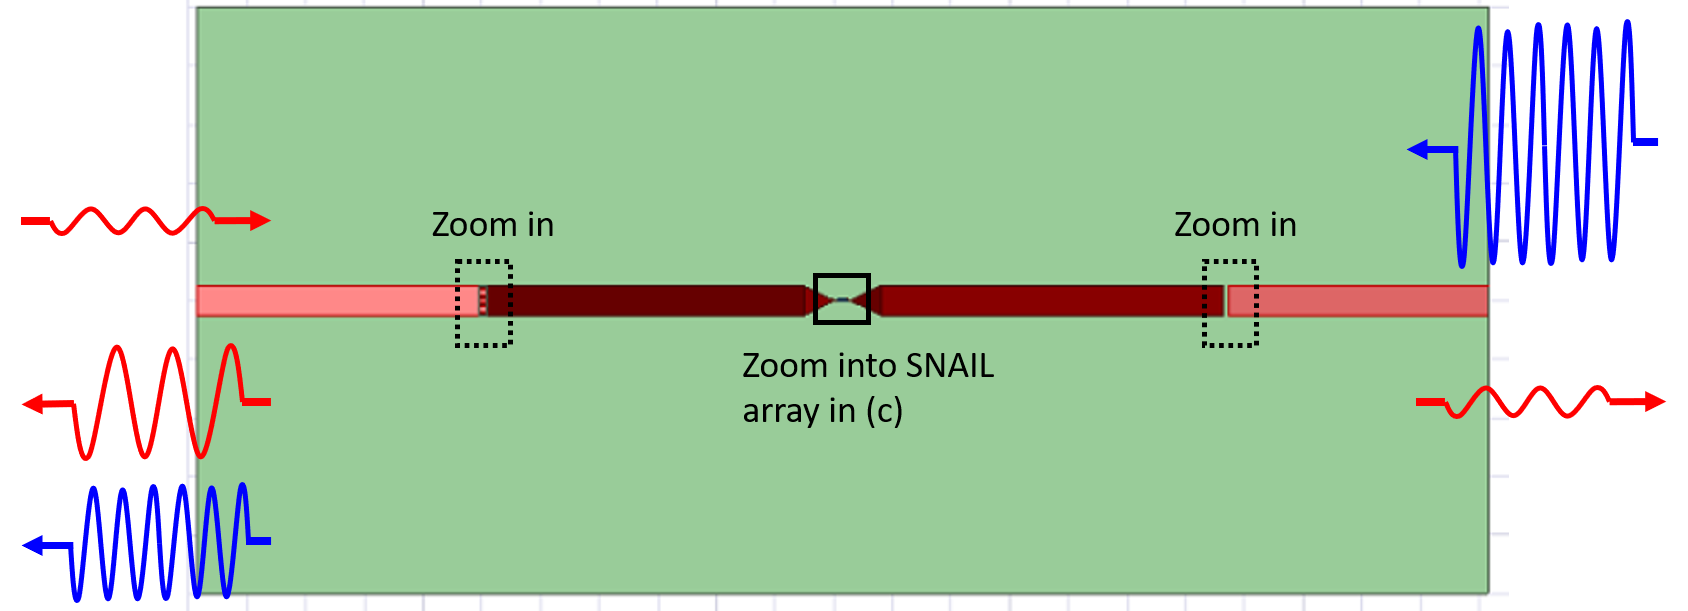
\includegraphics[width=6cm]{figures/SPA.PNG}
}
\subcaptionbox{filter coupled SPA}
{\label{fig:device2}
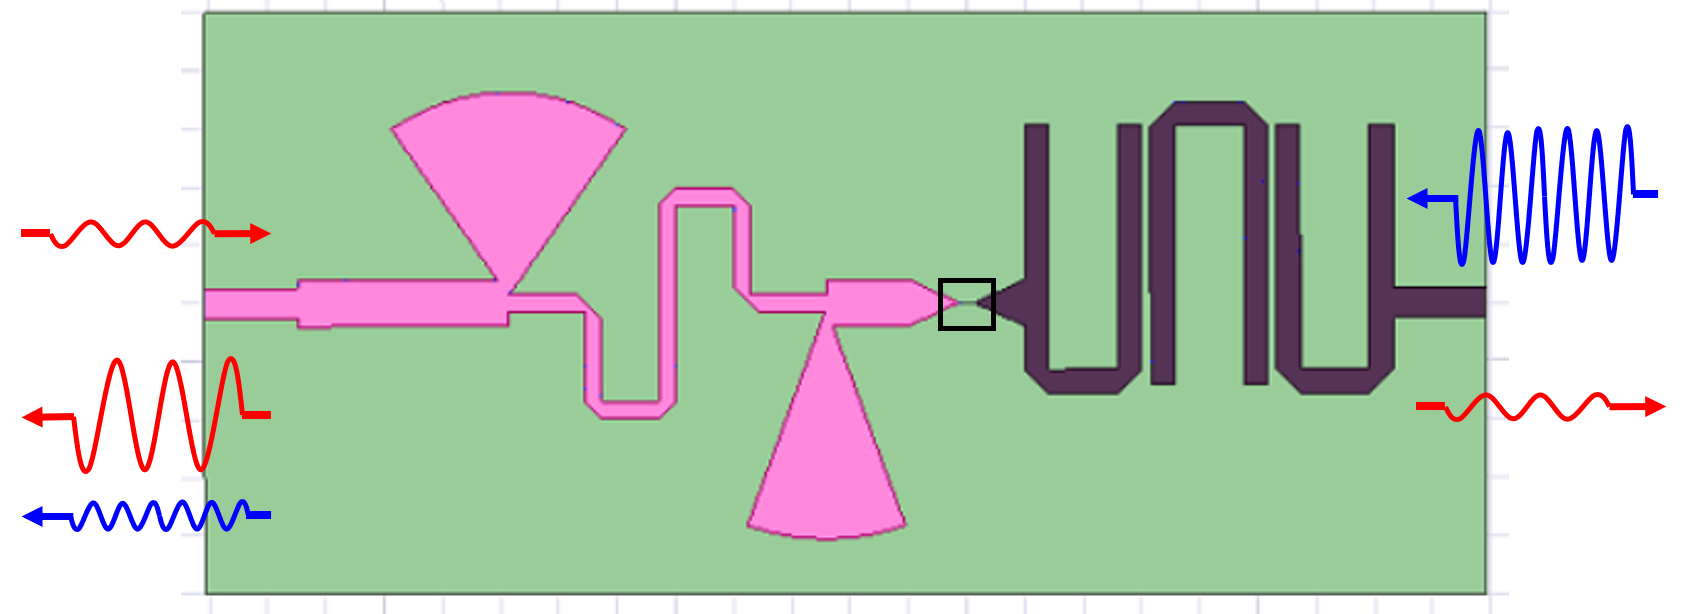
\includegraphics[width=6cm]{figures/FSPA.PNG}
}
\subcaptionbox{General circuit model: SPA with arbitrary linear network at both ports}
{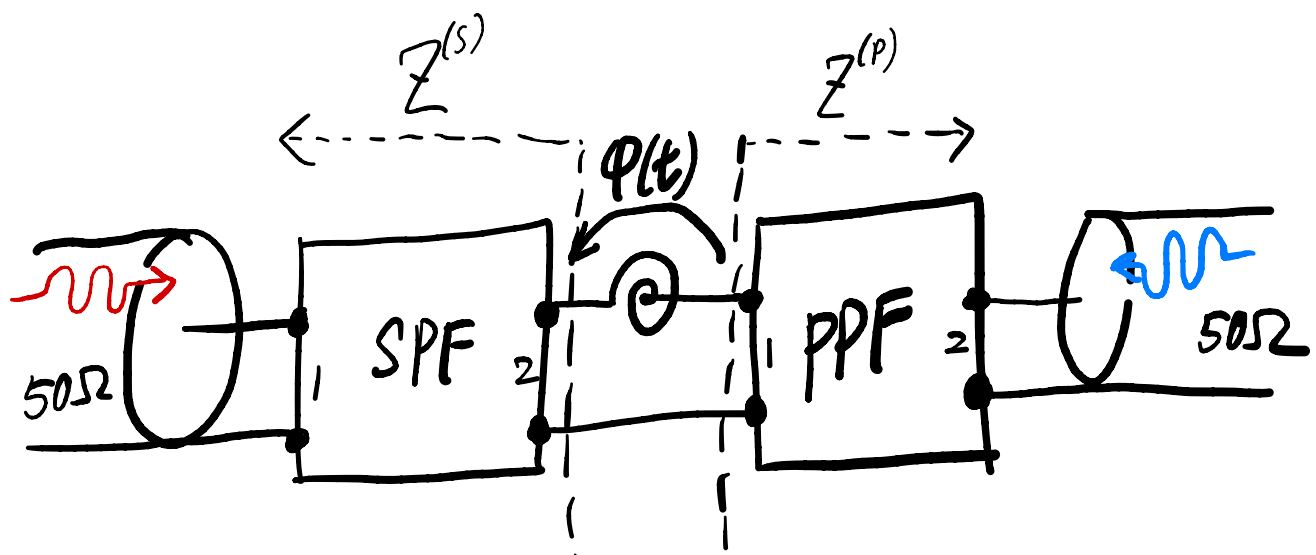
\includegraphics[width=12cm]{figures/SPA_diagram.jpg}
\label{fig:circuit_1} 
}
\caption
{\label{fig:device} Layout of a capacitively coupled SPA and a filter coupled SPA. Reflection gain is obtained from signal port, and minimal signal leakage from pump port is expected. Originally, different coupling capacitors are employed at signal and pump port. We suggest that a bandstop filter (pink) at signal port can suppress pump leakage while maintaining moderate signal coupling. And a bandpass filter (purple) at pump port provide strong coupling for pump and weak coupling for signal. }
\end{figure}

% Assume a linearized impedance $Z_J$ for the SNAIL array behaviour at drive frequency. 

A two-port SPA is formed by the concatenation of: 

signal port coupling network - SNAIL array - pump port coupling network

Most generally, the linear coupling networks can be described with S matrix. And if we assume for now the SNAIL array behave linearly, as an impedance $Z_J$, we can describe the SNAIL array also as a S matrix (evaluated assuming port impedance $Z_c$):
\[
S = 
\(
\begin{matrix}
R & T\\
T & R
\end{matrix}
\)
\]
with reflection and transmission coefficient respectively: 
\begin{equation}
R = \frac{Z_J}{Z_J+2 Z_c}
\end{equation}

\begin{equation}
T = \frac{2Z_c}{Z_J+2 Z_c}
\end{equation}


In SPA application, the external drive we apply is typically a CW tone at fixed frequency, injecting from either one of the two ports. For the case of interest in next section, let's take the pump ($\omega_p$ frequency component, incoming from pump port) as an example: 

From a signal flow chart analysis: 

When we inject CW tone pump voltage $V_p \cos(\omega_p t) = \Re \(V_p \exp{j \omega_p t}\) = \frac{V_p}{2} \exp{j \omega_p t} + \frac{V_p^*}{2} \exp{-j \omega_p t}$ into pump port: 

\begin{equation}
V_0 = \frac{S^{(p)}_{12} V_p/2}{1 - \( R + \frac{S^{(s)}_{22} T^2}{1- S^{(s)}_{22} R } \) S^{(p)}_{11}} 
\end{equation}

Overall voltages on the left and right node of the SNAIL array are, respectively: 

\begin{equation}
V_L = \frac{T}{1-S^{(s)}_{22} R} \( 1+ S^{(s)}_{22} \)V_0
\end{equation}

\begin{equation}
V_R = \( 1 + R + \frac{S^{(s)}_{22} T^2}{1- S^{(s)}_{22} R } \)V_0 
\end{equation}

So voltage across the SNAIL is simply $V_L - V_R$, which can be written into incoming wave voltage amplitude $V_p$. And there's an easy convertion between voltage and phase difference $\varphi_{\omega_p} = \frac{V_L - V_R}{j \omega_p}$. 

In next section, we'll view $\varphi_{\omega_p}$ as already-computed, and use it in the pumpistor model. 



\newpage

\section{Pumpistor model for current pumped SNAIL}\label{appen:SNAIL}

\subsection{SNAIL}

% The whole point of pumpistor model is to linearize a nonlinear parametric process, specifically parametric amplification. When using an amplifier in its linear amplification regime (which is typically the case in cQED application), we can always introduce a linear circuit including negative resistance to effectively describe the amplification behavior. 

% Such a linear circuit model shows its advantage when we want to synthesize an amplifier along with some complex linear networks, e.g. filters, impedance transformers, or hybrids. 

A SNAIL has a nonlinear potential in the form: 
\begin{equation}\label{eq:U}
U =E_j \( c_0 + \frac{c_2}{2!} \tilde{\varphi}^2 + \frac{c_3}{3!} \tilde{\varphi}^3 + \frac{c_4}{4!} \tilde{\varphi}^4 + \cdots\)
\end{equation}

where $\tilde{\varphi}(t) = \frac{\Phi_L(t) - \Phi_R(t)}{M\phi_0} - \varphi_\mathrm{min}$, is phase difference across each SNAIL expanded around the static minimum $\varphi_\mathrm{min}$ determined by external flux bias. Note that $c_2$, $c_3$, $c_4$... all dependents on external magnetic flux. 

Current flowing through a SNAIL is given by: 
\begin{equation}\label{eq:It}
I(t) = \frac{E_j}{\phi_0} \( c_2\tilde{\varphi} +  \frac{c_3}{2} \tilde{\varphi}^2  + \frac{c_4}{6} \tilde{\varphi}^3 + \cdots \)
\end{equation}

where $E_j$ is Josephson energy of the large junction* in a SNAIL. 

*\emph{Just as a reminder: a typical large junction (7um-long*700nm-wide Dolan bridge process) that we make has}
\begin{center}
\begin{tabular}{ c | c | c }
 $L_j$ (pH) & $E_j$ (GHz) & $I_c$ (uA) \\ 
 \hline
 50 & 1635 & 6.6    
\end{tabular}
\end{center}

In the following we treat such an array as one lumped element, and $\varphi$ stands for the phase difference across the whole SNAIL array. Total inductance of a SNAIL array consisting of M SNAILs should be: 
\begin{equation}
L_J = ML_j/c_2
\end{equation}



% In phase preserving amplification process, $\tilde{\varphi}(t)$ composes of only three frequency components, namely signal $\omega_s$, pump $\omega_p$ and idler $\omega_i = \omega_p - \omega_s$ (to be exact, it is the counter-rotating idle component, i.e. $- \omega_i$ that is of interest). 

\begin{figure}[htb]
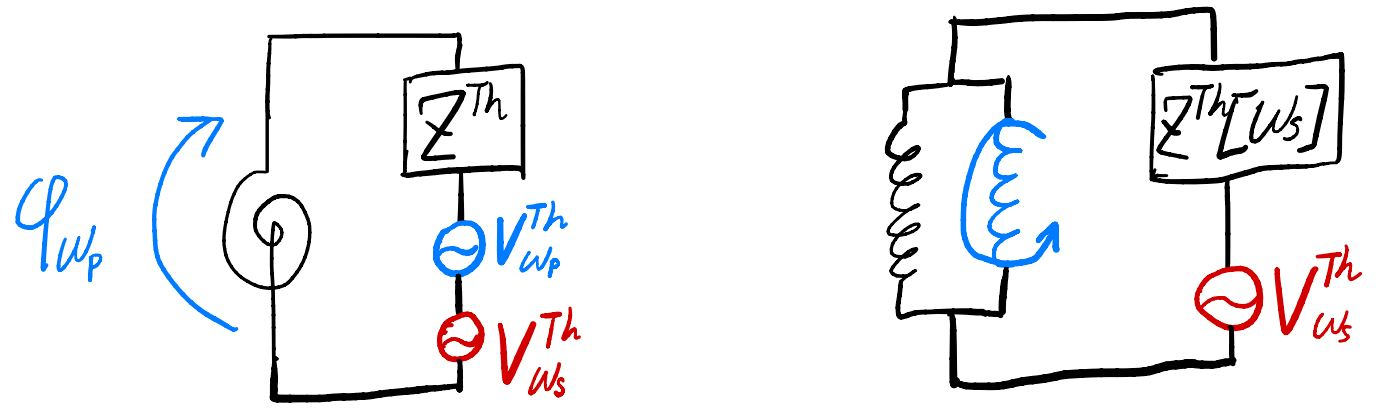
\includegraphics[width=12cm]{figures/Pumpistor.jpg}
\caption{Pumpsitor model: linearized impedance for a pumped SNAIL}
\end{figure}

\subsection{Pumpistor impedance considering $c_3$}

Consider only the first two terms in \eq{eq:It}, the $\exp{j\omega_s t}$ harmonic component of $I(t)$ will yield: 
\[
	I_{\omega_s} = \frac{I_c}{M} \(c_2 \varphi_{\omega_s} + \frac{c_3}{2} \varphi_{\omega_p} \varphi^*_{\omega_i}\) 
\]
($I_c = E_j/\phi_0$, is critical current of the large junction in a SNAIL. )


Put together

\begin{equation}\label{eq:IV}
\(
\begin{matrix}
I_{\omega_s}\\
I^*_{\omega_i}
\end{matrix}
\)
= 
\frac{1}{j L_J}
\(
\begin{matrix}
\frac{1}{\omega_s} & \frac{\epsilon}{-\omega_i}\\
\frac{\epsilon^*}{\omega_s} & \frac{1}{-\omega_i}
\end{matrix}
\)
\(
\begin{matrix}
V_{\omega_s}\\
V^*_{\omega_i}
\end{matrix}
\)
\end{equation}

and 

\begin{equation}
	I^*_{\omega_i} Z^\Th[-\omega_i] + V^*_{\omega_i} = 0*
\end{equation}

*\emph{Because in application, there's no external probe at $\omega_i$ (except for vacuum noise). }

We get the following relation: 
\begin{equation*}
	\frac{V^*_{\omega_i}}{V_{\omega_s}} = \frac{\epsilon^*}{\frac{\omega_s}{\omega_i} - \frac{j L_J \omega_s}{Z^\Th[-\omega_i]} } 
\end{equation*}

Thus, we can express the linearized response at $\omega_s$ as an overall impedance: 

\begin{equation}\label{eq:ZJ}
	Z_J[\omega_s] = \frac{j L_J \omega_s }{1 - \frac{\abs{\epsilon}^2}{1 - jL_J \omega_i/Z^{\Th^*}[\omega_i]}}
\end{equation}



\subsection{Pumpsitor impedance considering $c_3$ and $c_4$}

To get the renormalized Kerr coefficient (from 2nd order perturbation as shown in SPA paper) correctly, we have to include also the higher idler frequency $\omega_h = \omega_s + \omega_p = 2\omega_p - \omega_i $


\begin{equation}
	I_{\omega_s} = \frac{I_c}{M} \(c_2 \varphi_{\omega_s} + \frac{c_3}{2} \( \varphi_{\omega_p} \varphi^*_{\omega_i} + \varphi^*_{\omega_p} \varphi_{\omega_h}\) + \frac{c_4}{4} |\varphi_{\omega_p}|^2 \varphi_{\omega_s}\) 
\end{equation}


Let's consider the Kerr effect due to pump only, and denote: 
\begin{equation}
\delta = \frac{c_4}{4c_2}|\varphi_{\omega_p}|^2
\end{equation}

We get: 

\begin{equation}
\(
\begin{matrix}
I_{\omega_s}\\
I^*_{\omega_i}\\
I_{\omega_h}
\end{matrix}
\)
= 
\frac{1}{j L_J}
\(
\begin{matrix}
\frac{1 + \delta}{\omega_s} & \frac{-\epsilon}{\omega_i} & \frac{\epsilon^*}{\omega_h}\\
\frac{-\epsilon^*}{\omega_s} & \frac{1 + \delta}{\omega_i} & 0 \\
\frac{\epsilon}{\omega_s} & 0 & \frac{1 + \delta}{\omega_h}
\end{matrix}
\)
\(
\begin{matrix}
V_{\omega_s}\\
V^*_{\omega_i}\\
V_{\omega_h}
\end{matrix}
\)
\end{equation}

which should be put together with:

\begin{equation*}
\begin{aligned}
	I^*_{\omega_i} Z^\Th[-\omega_i] + V^*_{\omega_i} &= 0 \\
	I_{\omega_h} Z^\Th[\omega_h] + V_{\omega_h} &= 0
\end{aligned}
\end{equation*}

Consequently: 


\begin{equation*}
\begin{aligned}
	\frac{V^*_{\omega_i}}{V_{\omega_s}} &= \frac{\epsilon^*}{(1+\delta)\frac{\omega_s}{\omega_i} - \frac{j L_J \omega_s}{Z^\Th[-\omega_i]} } \\
	\frac{V_{\omega_h}}{V_{\omega_s}} &= \frac{-\epsilon}{(1+\delta)\frac{\omega_s}{\omega_h} + \frac{j L_J \omega_s}{Z^\Th[\omega_h]} }
\end{aligned}
\end{equation*}



So the overall linearized impedance at $\omega_s$ should be: 

\begin{equation}
	Z_J[\omega_s] = \frac{j L_J \omega_s }{1 + \delta - \frac{\abs{\epsilon}^2}{1 + \delta - jL_J \omega_i/Z^{\Th^*}[\omega_i]} - \frac{\abs{\epsilon}^2}{1 + \delta + jL_J \omega_h/Z^\Th[\omega_h]}}
\end{equation}



% While let us neglect $Z^\Th[\omega_h]$ for now (assuming it's a short). Keeping up to 1st order in $\delta$ and $\abs{\epsilon}^2$: 

% \begin{equation}
% Z_J[\omega_s] = \frac{j L_J (\omega_a + \Delta + \omega) \left[ (1+\delta) \( \frac{\kappa_a}{2} - j \frac{2}{p}(\Delta - \omega) \) + j \delta (\omega_a + \Delta - \omega)\right]}{(1 + 2\delta -\abs{\epsilon}^2) \( \frac{\kappa_a}{2} - j \frac{2}{p}(\Delta - \omega)\)] + j (\delta - \abs{\epsilon}^2) (\omega_a + \Delta - \omega)}
% \end{equation}


\newpage

\section{The case of resonance modes}\label{appen:mode}


\subsection{Why do we need a mode from the first place?}

For resonance parametric amplification (or more generally for any parametric process we're talking about), besides the Josephson element that provides nonlinearity, we also need one or several modes around the frequency components of interest. 

The only exception is the TWPA, where the parametric process happens for traveling waves instead of standing waves (steady state). 

In the photon scattering picture, the parametric process can be viewed as an elastic scattering between photons of different energy on the Josephson element. The reason we need a mode for the parametric process is simply to have a large density of state for the final state, resulting in a higher probability for this process to happen according to Fermi's golder rule. 



\subsection{What is a mode?}

% When talking about resonance condition, let's first keep only the linear part of \eq{eq:It}: 

% \begin{equation}\label{eq:LJ}
% I(t) = I_c c_2 \tilde{\varphi} = 
% \frac{\Phi_L(t) - \Phi_R(t) }{L_J} - M\phi_0\varphi_\min/L_J
% \end{equation}
In Doug's words: pure outgoing wave solution

A \emph{mode} stands for the eigenvalue (frequency) and eigenvector (field distribution function) for Maxwell Eqs with certain boundary condition, which I interprete as the 'undriven' EM field allowed in the system.

(Argue that there's only a discrete set of ${s_a}$ that satisfies: 
\[
Z^\Th[s_a] + s_a L_J = 0
\]


Assume the Josephson element has a linearized response $Z_J$, which behaves local in Laplace domain $t \rightarrow s$. 

Existance of non-trivial solutions for a system as shown in Figure. \ref{fig:Thevenin} requires that: 
\begin{equation}
	Z^\Th[s] + Z_J[s]= 0
\end{equation}

For the set of ${s_a}$ that satisfies the above relation, if we write $s_a = - \kappa_a/2 + j \omega_a$: 
\begin{align}
	\Im{Z^\Th[\omega_a]} &=  - \omega_a L_J \label{eq:R1}\\
	\Re{Z^\Th[\omega_a]} &=  \frac{\kappa_a}{2} L_J  \label{eq:R2}
\end{align}

General undriven solution to the system will be in the form of linear combination of eigenmodes: 
\begin{equation}
	I(t) = \sum_a I_{\omega_a} \exp{- \frac{\kappa_a}{2} t} \exp{j\omega_a t}
\end{equation}

*\emph{ Particularly in the case of an SPA, \eq{eq:R2} can be further written into: }
\begin{equation}
\Re{Z^{(s)}[\omega_a]} + \Re{Z^{(p)}[\omega_a]} =  \frac{\kappa_a}{2} L_J
\end{equation}

\emph{where we want the SPA mode linewidth to be dominated by signal port coupling, and leakage via pump port coupling to be minimal, 
i.e. $\Re Z^{(s)}[\omega_a]= \frac{\kappa_a}{2}L_J$, $\Re Z^{(p)}[\omega_a] \approx 0$
}



\subsection{Participation ratio of a Josephson element in a mode}


Apart from HFSS simulation, it will be useful to express 'participation ratio' in a closed-form expression. 

It turns out participation ratio of a lumped element can be defined using the 1st order derivative of output impedance it sees. 

\begin{equation}\label{eq:m}
m:= \frac{\Im Z^{\Th'}[\omega_a]}{L_J} = \frac{2L - L_J}{L_J}
\end{equation}

participation ratio: 
\begin{equation}
p:= \frac{L_J}{L} = \frac{2}{m + 1}
\end{equation}


\subsection{$Z_J[\omega_s]$ in the case of degenerate 3WM amplifier}
In a degenerate 3WM amplifier, both signal $\omega_s$ and idler $\omega_i$ are near resonance frequency $\omega_a$. Let's introduce some notions first:

Pump frequency: $\omega_p = 2 (\omega_a + \Delta)$

Signal frequency: $\omega_s = \omega_p/2 + \omega = \omega_a + \Delta + \omega$

Idler frequency: $\omega_i = \omega_p - \omega_s = \omega_a + \Delta - \omega$

Assume $\Re{Z^\Th}$ being flat, and include 1st order derivative of $\Im{Z^\Th}$, we get:
\begin{equation}\label{eq:ZE}
\begin{aligned}
Z^\Th[\omega_s] &= \frac{\kappa_a}{2}L_J - j \omega_a L_J + j m L_J (\Delta + \omega) \\
Z^{\Th^*}[\omega_i] &= \frac{\kappa_a}{2}L_J + j \omega_a L_J - j m L_J (\Delta - \omega)
\end{aligned}
\end{equation}
and 

In this case, the linearized impedance of SNAIL array in \eq{eq:ZJ} can be written as: 
\begin{equation}\label{eq:ZJ'}
\begin{aligned}
	Z_J[\omega_s] &= \frac{j L_J \omega_s }{1 - \frac{\abs{\epsilon}^2}{1 - jL_J \omega_i/Z^{\Th^*}[\omega_i]}}\\
	&= \frac{j L_J (\omega_a + \Delta + \omega) \left[ \frac{\kappa_a}{2} - j \frac{2}{p}(\Delta - \omega)\right]}{(1-\abs{\epsilon}^2)\left[ \frac{\kappa_a}{2} - j \frac{2}{p}(\Delta - \omega)\right] - j \abs{\epsilon}^2 (\omega_a + \Delta - \omega)} \\
	&\approx \frac{j L_J (\omega_a + \Delta + \omega) \left[ \frac{\kappa_a}{2} - j \frac{2}{p}(\Delta - \omega)\right]}{\frac{\kappa_a}{2} - j \frac{2}{p}(\Delta - \omega) - j \abs{\epsilon}^2 \omega_a }
\end{aligned}
\end{equation}



\newpage

\section{Evaluate SPA reflection coefficient}\label{appen:S11}

Recall that the reflection and transmission coefficients (in S-matrix) for a lumped impedance $Z_J$ is: 
\[
R = \frac{Z_J}{Z_J+2 Z_c} \qquad
T = \frac{2Z_c}{Z_J+2 Z_c}
\]
As the effective impedance for a pumped SNAIL array is derived in \eq{eq:ZJ}, it applies directly into the concatenated SPA: 

\begin{equation}
V_0 = \frac{S^{(s)}_{21} V_s}{1 - \( R + \frac{S^{(p)}_{11} T^2}{1- S^{(p)}_{11} R } \) S^{(s)}_{22}} 
\end{equation}



Overall reflection coefficient of the SPA is given by: 
\begin{equation}\label{eq:S11}
\frac{V_\out}{V_\in} = S^{(s)}_{11} + \frac{S^{(s)}_{21} S^{(s)}_{12} \Gamma }{1 - \Gamma S^{(s)}_{22}} 
\end{equation}
where we name:
\begin{equation}\label{eq:Gamma}
\begin{aligned}
\Gamma &=  R + \frac{S^{(p)}_{11} T^2}{1- S^{(p)}_{11} R } \\
% &= \frac{Z_J}{Z_J+2 Z_c} + \frac{  \frac{Z^{(p)}-Z_c}{Z^{(p)}+Z_c} \( \frac{2Z_c}{Z_J+2 Z_c} \)^2}{1-\frac{Z^{(p)}-Z_c}{Z^{(p)}+Z_c} \frac{Z_J}{Z_J+2 Z_c}}\\
% &=\frac{1}{Z_J + 2Z_c} \( Z_J + \frac{2Z_c}{\frac{Z_J+2Z_c}{Z^{(p)} -Z_c}+1} \)\\
&= \frac{Z_J + Z^{(p)} - Z_c}{Z_J + Z^{(p)} + Z_c}
\end{aligned}
\end{equation}
in which we have introduced pump port output impedance (seen by the SNAIL array): 
\[
Z^{(p)} = Z_c \frac{1 + S^{(p)}_{11}}{1- S^{(p)}_{11}}
\]
Similarly, signal port output impedance (seen by the SNAIL array) should be: 
\[
Z^{(s)} = Z_c \frac{1 + S^{(s)}_{22}}{1- S^{(s)}_{22}}
\]

In that case, the total external impedance $Z^\Th[\omega]$ seen by the SNAIL array would compose of: 
\begin{equation}
Z^\Th = Z^{(s)} + Z^{(p)}
\end{equation}

And \eq{eq:S11} is equivalent to: 
\begin{equation}\label{eq:S11'}
\begin{aligned}
\frac{V_\out}{V_\in} &= S^{(s)}_{11} + {S^{(s)}_{21}}{S^{(s)}_{12}} \frac{(Z^{(s)} + Z_c)(Z_J + Z^{(p)} - Z_c)}{2Z_c(Z_J + Z^{(s)} + Z^{(p)})} \\
&= S^{(s)}_{11} + {S^{(s)}_{21}}{S^{(s)}_{12}} \frac{Z^{(s)} + Z_c}{2Z_c} \( 1 - \frac{Z^{(s)} + Z_c}{Z_J + Z^\Th}\)
\end{aligned}
\end{equation}

Such a signal port filter network should be reciprocal: $S^{(s)}_{12} = S^{(s)}_{21}$ and unitary: $S^{(s)\dagger} S^{(s)} = I$ (assuming lossless). 

After some math, we have $S^{(s)}_{11}S^{(s)}_{22} - S^{(s)2}_{21} = \exp{j \theta}$ where $S^{(s)}_{11} = \exp{j \theta} S^{(s)*}_{22}$

% $\abs{S^{(s)}_{11}}^2 + \abs{S^{(s)}_{21}}^2 = \abs{S^{(s)}_{21}}^2 + \abs{S^{(s)}_{22}}^2 = 1$

Plug into \eq{eq:S11'}: 
\begin{equation*}
\begin{aligned}
\frac{V_\out}{V_\in} &= \exp{j \theta} S^{(s)*}_{22} + \exp{j \theta} \(\abs{S^{(s)}_{22}}^2 - 1\)
\frac{Z^{(s)} + Z_c}{2Z_c} \( 1 - \frac{Z^{(s)} + Z_c}{Z_J + Z^\Th} \) \\
&= \exp{j \theta} \left[ 
\frac{Z^{(s)*} - Z_c}{Z^{(s)*} + Z_c} + 
\(
\abs{\frac{Z^{(s)} - Z_c}{Z^{(s)} + Z_c}}^2 - 1
\)
\frac{Z^{(s)} + Z_c}{2Z_c} \( 1 - \frac{Z^{(s)} + Z_c}{Z_J + Z^\Th} \)
\right]\\
&= \exp{j \theta} \left[ 
\frac{Z^{(s)*} - Z_c}{Z^{(s)*} + Z_c} + 
\(
\frac{\abs{Z^{(s)} - Z_c}^2 - \abs{Z^{(s)} + Z_c}^2}{(Z^{(s)} + Z_c)(Z^{(s)*} + Z_c)}
\)
\frac{Z^{(s)} + Z_c}{2Z_c} \( 1 - \frac{Z^{(s)} + Z_c}{Z_J + Z^\Th} \)
\right]\\
&= \frac{\exp{j \theta}}{Z^{(s)*} + Z_c} \left[ 
Z^{(s)*} - Z_c + 
\frac{-4 \Re Z^{(s)} Z_c}{2Z_c}
\( 1 - \frac{Z^{(s)} + Z_c}{Z_J + Z^\Th} \)
\right] \\
&= \frac{\exp{j \theta}}{Z^{(s)*} + Z_c} \left[ 
Z^{(s)*} - 2\Re Z^{(s)} - Z_c + 2 \Re Z^{(s)}
\frac{Z^{(s)} + Z_c}{Z_J + Z^\Th}
\right] \\
&= \exp{j \theta}\frac{Z^{(s)} + Z_c}{Z^{(s)*} + Z_c} 
\(\frac{2\Re Z^{(s)}}{Z_J + Z^\Th} - 1 \)
\end{aligned}
\end{equation*}


\subsection{No pump: linear mode phase roll and linewidth}

Specifically, $Z_J[\omega_s] = j L_J (\omega_a + \Delta + \omega)$ without pump (i.e. when $\epsilon = 0$). In this case: 

\begin{equation}
\begin{aligned}
\frac{V_\out[\omega_s]}{V_\in[\omega_s]} &= \exp{j \theta}\frac{Z^{(s)}[\omega_s] + Z_c}{Z^{(s)*}[\omega_s] + Z_c} 
\(\frac{\kappa_a}{\frac{\kappa_a}{2} + j\frac{2}{p} (\omega_s - \omega_a)} - 1 \)\\ 
&= \exp{j (\theta + 2\theta_{\omega_s})}
\frac{\frac{p}{2}\frac{\kappa_a}{2} + j(\omega_s - \omega_a)}{\frac{p}{2}\frac{\kappa_a}{2} - j(\omega_s - \omega_a)}
\end{aligned}
\end{equation}
Here $\theta_{\omega_s}$ is phase factor of $\Re Z^{(s)}[\omega_s] + Z_c + j \Im Z^{(s)}[\omega_s]$, which should be smooth over frequency. So we can take it as adding an overall slope on the phase roll. 


\subsection{Gain}

If we look at power gain $G[\omega] = \abs{\frac{V_\out[\omega]}{V_\in[\omega]}}^2$: 
\begin{equation}
\begin{aligned}
G[\omega_s] &=  
\abs{\frac{2\Re Z^{(s)}[\omega_s]}{Z_J[\omega_s] + Z^\Th[\omega_s]} - 1}^2\\
&= \abs{ \frac{\kappa_a}{\frac{Z_J[\omega_s]}{L_J} + \frac{\kappa_a}{2} - j (\omega_a - m (\Delta + \omega))} - 1 }^2
\end{aligned}
\end{equation}

Recall from \eq{eq:ZJ'} that the pumped SNAIL array has effective impedance: 

\begin{equation}
	Z_J[\omega_s] \approx \frac{j L_J (\omega_a + \Delta + \omega) \left[ \frac{\kappa_a}{2} - j \frac{2}{p}(\Delta - \omega)\right]}{\frac{\kappa_a}{2} - j \frac{2}{p}(\Delta - \omega) - j \abs{\epsilon}^2 \omega_a }
\end{equation}

Plug this into the above equation, we get: 

\begin{equation*}
G = 1 + \frac{\kappa_a^2 \abs{\epsilon}^2 [(\omega_a + \Delta)^2 - \omega^2]}{(1+m)^2\kappa_a^2\omega^2 + 
\(\frac{\kappa_a^2}{4} + \Delta^2 (1+m)^2  - \omega^2 (1+m)^2 + 2m\abs{\epsilon}^2 \Delta \omega_a - \abs{\epsilon}^2 \omega_a^2
\)^2}
\end{equation*}

After some maths and relabeling, it ends up in a prettier form: 

\begin{equation}
G = 1 + \frac{\kappa^2 \abs{\epsilon' \omega_p/2}^2 }{\kappa^2\omega^2 + 
\(\frac{\kappa^2}{4} + \Delta^2 - \omega^2 - \abs{\epsilon' \omega_p/2}^2
\)^2}
\end{equation}


Maximum gain is obtained when signal detuning $\omega \approx 0$: 
\begin{equation}
G_0 = 1 + \frac{\kappa^2 \abs{\epsilon' \omega_p/2}^2 }{
\(\frac{\kappa^2}{4} + \Delta^2 - \abs{\epsilon' \omega_p/2}^2
\)^2}
\end{equation}

where $\epsilon' = \frac{\epsilon}{1+m} = \frac{p c_3\varphi_{\omega_p}}{4c_2}$, $\kappa = \frac{\kappa_a}{1+m} = \frac{p}{2}\kappa_a$

\subsection{Verification: A lumped SPA}

Impedance seen by the SNAIL: 

\begin{equation*}
Z^\Th[\omega_s] = \frac{R}{1 + j \omega_s RC} + j \omega_s L
\end{equation*}

We can evaluate its real and imaginary part respectively:
\begin{equation*}
\begin{aligned}
\Re Z^\Th[\omega_s] &= \frac{R}{1 + \omega_s^2 R^2C^2} \\
& \approx \frac{1}{\omega_s^2 R C^2} \(1- \frac{1}{\omega_s^2 R^2 C^2}\) \\
& \approx \frac{1}{\omega_a^2 R C^2} \( 1 - \frac{2\Delta}{\omega_a} \) \(1- \frac{1}{\omega_a^2 R^2 C^2}\) \\
&= \frac{L_J + L}{R C} \( 1 - \frac{2\Delta}{\omega_a} \) \(1- \frac{Z_a^2}{R^2}\)
\end{aligned}
\end{equation*}

\begin{equation*}
\begin{aligned}
\Im Z^\Th[\omega_s] &= \omega_s L - \frac{\omega_s R^2 C}{1 + \omega_s^2 R^2C^2} \\
& \approx \omega_s \(L - \frac{1}{\omega_s^2 C} \(1- \frac{Z_a^2}{R^2}\) \) \\
& \approx (\omega_a + \Delta) \(L - (L_J + L) \(1- \frac{2\Delta}{\omega_a} \) \) \\
&= -\omega_a L_J + L_J \(\frac{2L}{L_J}+1\)\Delta
\end{aligned}
\end{equation*}

According to the relations in Section \ref{appen:mode}

\begin{equation*}
\Im Z^\Th[\omega_a] = -\omega_a L_J
\end{equation*}

\begin{equation*}
m = \frac{\Im Z^\Th[\omega_a]}{L_J} = \frac{2L}{L_J} + 1
\end{equation*}

And we see that SNAIL participation ratio is: 

\begin{equation*}
p = \frac{2}{m+1} = \frac{L_J}{L + L_J}
\end{equation*}

\begin{equation*}
\kappa = \frac{p}{2} \kappa_a = \frac{L_J}{2(L + L_J)} \frac{2 \Re Z^\Th[\omega_a]}{L_J} = \frac{1}{RC}
\end{equation*}


\newpage

\section{Impedance engineered broadband JPA}

In previous section, we have already shown that the gain profile has a frequency (signal detuning from $\omega_p/2$) dependence: 
\begin{equation*}
G[\omega] \approx \frac{\kappa^2 \abs{\epsilon' \omega_p/2}^2 }{\kappa^2\omega^2 + 
\(\frac{\kappa^2}{4} + \Delta^2 - \omega^2 - \abs{\epsilon' \omega_p/2}^2
\)^2}
\end{equation*}

When using a JPA, we usually talk about its gain at the peak, i.e. at $\omega \approx 0$: 
\begin{equation*}
G_0 \approx \frac{\kappa^2 \abs{\epsilon' \omega_p/2}^2 }{
\(\frac{\kappa^2}{4} + \Delta^2 - \abs{\epsilon' \omega_p/2}^2
\)^2}
\end{equation*}

After some maths, we get: 
\begin{equation}
G[\omega] = \frac{G_0}{1 + (\omega/\Gamma)^2}
\end{equation}
where the dynamical bandwidth of the amplifier:
\begin{equation}\label{eq:GainBW}
\Gamma = \frac{1}{\sqrt{G_0}} \frac{\kappa \abs{\epsilon' \omega_p/2}}{\sqrt{2 \(\frac{\kappa^2}{4} - \Delta^2 + \abs{\epsilon' \omega_p/2}^2
\)}}
\end{equation}

Worth noting, in the case of zero pump detuning ($\Delta \approx 0$) and high gain ($\frac{\kappa^2}{4} + \Delta^2 - \abs{\epsilon' \omega_p/2}^2 \approx 0$), \eq{eq:GainBW} have a prettier looking: 

\begin{equation}\label{eq:GainBW}
2\Gamma = \frac{\kappa}{\sqrt{G_0}}
\end{equation}
i.e. FWHM in gain profile is approximately resonance linewidth $\kappa$ over root gain. This is the famous gain-bandwidth tradeoff. 



According to literature, engineering a slope in the real part of output impedance could made a broadband JPA beyond the gain-bandwidth tradeoff. 

As a reminder, previously in \eq{eq:ZE} we're assuming the real part of output impedance being constant around $\omega_a$ (i.e. the slope being negligible). 

Now we want to include the 

\begin{equation}
Z^\Th[\omega_s]= \frac{\kappa_a}{2}L_J + r L_J (\omega_s - \omega_a) - j \omega_a L_J + j m L_J (\omega_s - \omega_a)
\end{equation}

where we're assuming $\Re Z^{(p)}[\omega_a] = \Re Z^{(p)'}[\omega_a] = 0$ and: 
\begin{equation}\label{eq:r}
r:= \frac{\Re Z^{(s)'}[\omega_a]}{L_J}
\end{equation}


In this case: 
\begin{equation}
\begin{aligned}
G[\omega_s] &=  
\abs{\frac{2\Re Z^{(s)}[\omega_s]}{Z_J[\omega_s] + Z^\Th[\omega_s]} - 1}^2\\
&= \abs{ \frac{\kappa_a + 2r (\Delta + \omega)}{\frac{Z_J[\omega_s]}{L_J} + \frac{\kappa_a}{2} + r(\Delta + \omega) - j (\omega_a - m (\Delta + \omega))} - 1 }^2
\end{aligned}
\end{equation}

And
\begin{equation}
	Z_J[\omega_s] = \frac{j L_J (\omega_a + \Delta + \omega) \left[ \frac{\kappa_a}{2} + r(\Delta - \omega) - j \frac{2}{p}(\Delta - \omega)\right]}{\frac{\kappa_a}{2} + r(\Delta - \omega) - j \frac{2}{p}(\Delta - \omega) - j \abs{\epsilon}^2 \omega_a}
\end{equation}

Like what we did in section \ref{appen:S11}, let's start with the case of no pump: $Z_J[\omega_s] = j L_J \omega_s$ 

\begin{equation*}
\begin{aligned}
\frac{V_\out[\omega_s]}{V_\in[\omega_s]} &= \exp{j \theta}\frac{Z^{(s)}[\omega_s] + Z_c}{Z^{(s)*}[\omega_s] + Z_c} 
\(\frac{\kappa_a + 2r(\omega_s - \omega_a) }{\frac{\kappa_a}{2} + r(\omega_s - \omega_a) + j(m+1)(\omega_s - \omega_a)} - 1 \)\\ 
&= \exp{j (\theta + 2\theta_{\omega_s})}
\frac{\frac{p}{2}\(\frac{\kappa_a}{2} + r(\omega_s - \omega_a)\) + j(\omega_s - \omega_a)}{\frac{p}{2} \(\frac{\kappa_a}{2} + r(\omega_s - \omega_a)\) - j(\omega_s - \omega_a)}
\end{aligned}
\end{equation*}

(And what does this imply? )




\begin{equation*}
G = 1 + \frac{ (\kappa_a + 2 r (\Delta + \omega)) (\kappa_a + 2 r (\Delta - \omega)) \abs{\epsilon}^2 [(\omega_a + \Delta)^2 - \omega^2]}{ \omega^2 \( (1+m)\kappa_a - 2r \abs{\epsilon}^2 \omega_a \)^2 +
\(\frac{\kappa_a^2}{4} + \Delta^2 (1+m)^2  - \omega^2 (1+m)^2 - \abs{\epsilon}^2 \omega_a^2 + r^2 (\Delta^2 - \omega^2) + r \Delta \kappa_a
\)^2}
\end{equation*}


\begin{equation}
G = 1 + \frac{ \(\kappa'^2 - (p\omega/2)^2 \)\abs{\epsilon' \omega_p/2}^2}{ \omega^2  (\kappa^2 - 4r \kappa \abs{\epsilon'}^2 \omega_a) +
\( \frac{\kappa'^2}{4} + \Delta^2 - (1+r^2) \omega^2 - \abs{\epsilon' \omega_p/2}^2) 
\)^2}
\end{equation}

where $\kappa' = \kappa + p r \Delta = \frac{\kappa_a + 2r\Delta}{m+1}$

In the high gain case, the denominator is close to zero, and slight drifting on the denominator would results in significant gain drop. 

Therefore, even though $\omega$ enter both numerator and denominator in the gain expression, we want the denominator to be lowest-order-independent of $\omega$. i.e.

\begin{equation}
(\kappa^2 - 4r \kappa \abs{\epsilon'}^2 \omega_a) -
2(1+r^2) \( \frac{\kappa'^2}{4} + \Delta^2 - \abs{\epsilon' \omega_p/2}^2) 
\) = 0
\end{equation}




\subsection{An ideal resonant paramp}

\begin{itemize}
	\item{Working at Kerr-free point (with certain pump detuning)}
	\item{Impedance transformer designed according to this particular pump detuning}
	\item{Pump delivery being efficient}
	\item{Minimal pump leakage towards signal port}
	\item{Being broadband around the Kerr-free working point}
\end{itemize}

We really need to get the denominator close to zero. 

If we dilute nonlinearity $g_3$, we need to pump harder. 

If we introduce pump tone detuning (from twice resonance, which is typically the easiest point to pump), we need to pump harder. 

In the easiest case, required $\varphi_{\omega_p}$ depends on $\kappa$ and 3rd order nonlinearity (which is proportional to participation ratio of the Josephson element in the mode). 

We can play with the impedances, 


\emph{a list of things to discuss}
\begin{itemize}
	\item{In order to readout harder, both compression power and dynamical bandwidth need to be improved. (Question for Zhixin?)}
	\item{Full Hamiltonian Controled JPC also require stronger pump than normal (because of lower participation ratio? And they're off resonant anyway)	(Question for Gangqiang?)}
\end{itemize}



If we simply use larger $\kappa$, we run into pQ limit (i.e. as we require larger $\varphi_{\omega_p}$ across the Josephson element, it become closer to 1 (critical current), higher order effects becomes non-negligible)

Required $\abs{\varphi_{\omega_p}}^2$ is proportional to $\kappa^2$, and compression power in both Kerr and pump depletion cases are also proportional to $\kappa^2$. So the ratio between them are somewhat fixes versus $\kappa$. 



High gain, doesn't sacrafice any information in the case of dispersive readout


\newpage

\section{Gain compression}

A reminder for the degenerate 3WM amplifier notations:

Pump frequency: $\omega_p = 2 (\omega_a + \Delta)$

Signal frequency: $\omega_s = \omega_p/2 + \omega = \omega_a + \Delta + \omega$

Idler frequency: $\omega_i = \omega_p - \omega_s = \omega_a + \Delta - \omega$

As we've already shown, peak gain of a JPA is achieved when $\omega \approx 0$: 

\begin{equation}
G_0 = 1 + \frac{\kappa^2 \abs{\epsilon' \omega_p/2}^2 }{
\(\frac{\kappa^2}{4} + \Delta^2 - \abs{\epsilon' \omega_p/2}^2
\)^2}
\end{equation}

Recall that the mode frequency $\omega_a$ and linewidth $\kappa$ are given by certain expressions including $Z^\Th$ and bare Josephson inductance $L_J$. 




\newpage

\section{Noise}


\begin{equation*}
\begin{aligned}
\mathrm{NVR} &= P_{\mathrm{on}}/P_{\mathrm{off}}\\
&= \frac{G_\sys(T_\sys+G(T_Q+T_{\mathrm{add}}))}{G_\sys(T_\sys+T_Q)}\\
&= \frac{G}{T_\sys+T_Q}T_\mathrm{add} + \frac{T_\sys+G T_Q}{T_\sys+T_Q}
\end{aligned}
\end{equation*}

\begin{equation*}
\begin{aligned}
\mathrm{NVR^*} &= \frac{G^*}{T_\sys+T_Q} (T_Q + k T_N) + \frac{T_\sys+G^* T_Q}{T_\sys+T_Q}\\
&= \frac{k}{T_\sys + T_Q} G^* T_N + \frac{T_\sys + 2 G^* T_Q}{T_\sys + T_Q}
\end{aligned}
\end{equation*}

\begin{equation*}
\begin{aligned}
\mathrm{NVR^*} &= \frac{G_\sys(T_\sys+G(T_Q+T^*_{\mathrm{add}}))}{G_\sys(T_\sys+T_Q)}\\
&= \frac{G}{T_\sys+T_Q}T^*_\mathrm{add} + \frac{T_\sys+G T_Q}{T_\sys+T_Q}
\end{aligned}
\end{equation*}



\[
T_\mathrm{add} = T_Q + k T_N
\]

\[
\mathrm{NVR} = \frac{k}{T_\sys} GT_N + \mathrm{NVR}_0
\]

\[
\mathrm{NVR}_0 = \frac{T_\sys + 2 G T_Q}{T_\sys + T_Q}
\]

\end{document}